\begin{table}[ht]
\centering\small
\begin{tabular}{lrrrrrrr}
\toprule
& Valid & \multicolumn{3}{c}{Originals (32)} & \multicolumn{2}{c}{Diagnostics (32)} & Paired\\
Method & /64 & Keep & Review & Reject & Reject & Review & /32\\
\midrule
Zero-shot & 64 & 25 & 5 & 2 & 27 & 5 & 20 \\
Few-shot & 64 & 27 & 4 & 1 & 25 & 7 & 21 \\
Stepwise CoT & 64 & 25 & 5 & 2 & 25 & 7 & 20 \\
Agent & 63 & 27 & 4 & 1 & 27 & 4 & 23 \\
No feedback & 63 & 27 & 4 & 1 & 27 & 4 & 22 \\
\bottomrule
\end{tabular}
\caption{Held-out results, using fixed denominators. No method kept a diagnostic. Each agent condition has one invalid diagnostic (excluded from reject/review counts but retained in denominators). Paired means keep original and reject its paired defect; originals are not gold positives.}\label{tab:quality}
\end{table}

\paragraph{Quality tradeoffs.} Zero-shot rejected 27/32 diagnostics (84.4\%) and kept 25/32 originals (78.1\%). Few-shot kept two more originals but rejected two fewer diagnostics. Stepwise prompting matched zero-shot original decisions exactly and moved two repetitive diagnostics from reject to review. The agent kept 27/32 originals and rejected 27/32 diagnostics, with the highest paired count (23/32, 71.9\%). That count does not establish better natural-data accuracy: it rewards original retention without gold quality labels. All five strict-policy subsets excluded every diagnostic; the unresolved distinction was often rejection versus review.

\paragraph{Which defects were difficult?} Every method rejected all eight empty, eight unrelated, and eight instruction-echo outputs. Differences occurred on excessive repetition (Figure~\ref{fig:repeat}). Review rather than reject can reflect a clarity score of 1, even when the explanation notices the repetition. This is a threshold/severity issue, not necessarily failure to notice the defect.

\begin{figure}[ht]
\centering
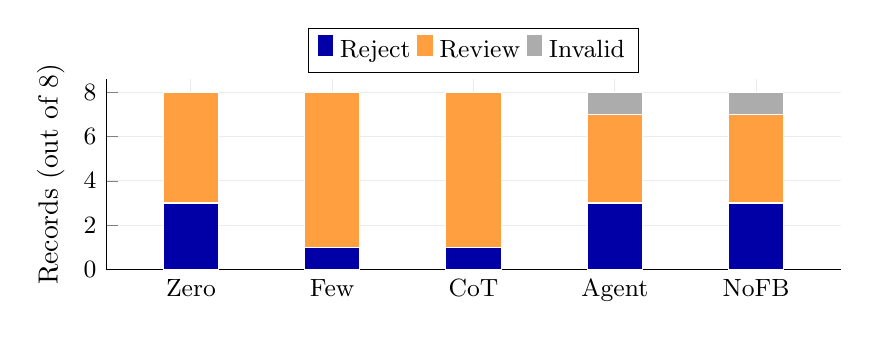
\begin{tikzpicture}
\begin{axis}[ybar stacked,width=.9\linewidth,height=4.0cm,
 ymin=0,ymax=8.6,ytick={0,2,4,6,8},ylabel={Records (out of 8)},
 symbolic x coords={Zero,Few,CoT,Agent,NoFB},xtick=data,
 bar width=20pt,enlarge x limits=.15,
 legend style={at={(.5,1.03)},anchor=south,legend columns=3,font=\small},
 axis lines*=left,tick label style={font=\small},grid=major,grid style={gray!15}]

\addplot[fill=blue!65!black,draw=white] coordinates {(Zero,3) (Few,1) (CoT,1) (Agent,3) (NoFB,3)};
\addplot[fill=orange!75,draw=white] coordinates {(Zero,5) (Few,7) (CoT,7) (Agent,4) (NoFB,4)};
\addplot[fill=gray!65,draw=white] coordinates {(Zero,0) (Few,0) (CoT,0) (Agent,1) (NoFB,1)};
\legend{Reject,Review,Invalid}
\end{axis}
\end{tikzpicture}
\caption{Outcomes on eight fourfold-repetition diagnostics. No repetition record was kept. NoFB denotes the agent without inspection observations.}\label{fig:repeat}
\end{figure}

\paragraph{Agent and ablation.} The agent inspected 18/64 records; the ablation inspected 17/64. No reassess action was observed and neither used a third call. The instruction to inspect was a prompt policy, not a runtime-enforced rule: both variants skipped three records whose actual whitespace word counts exceeded 120 (123, 124, and 131 words). The agent and ablation had identical aggregate keep/review/reject/failure counts, but differed on three diagnostic decisions and one paired success. One agent finish and one ablation finish omitted a closing JSON brace. Their plausible-looking assessments remain invalid, rather than being repaired after observing test results. The evidence supports an active feedback loop, but not a reliable overall benefit from feedback.

\begin{table}[ht]
\centering\small
\begin{tabular}{lrrrrrr}
\toprule
Method & Calls & Input tokens & Output tokens & Mean s & Median s & CNY\\
\midrule
Zero-shot & 64 & 34,519 & 5,259 & 1.40 & 1.34 & 0.1111 \\
Few-shot & 64 & 47,191 & 4,470 & 1.28 & 1.25 & 0.1301 \\
Stepwise CoT & 64 & 37,655 & 5,419 & 1.39 & 1.34 & 0.1187 \\
Agent & 82 & 78,286 & 6,655 & 1.80 & 1.56 & 0.2098 \\
No feedback & 81 & 76,100 & 6,560 & 1.77 & 1.50 & 0.2047 \\
\bottomrule
\end{tabular}
\caption{All 64 terminal records per method, including invalid outputs. Request latency is summed within a record. Costs use conservative list rates and include failed-format calls.}\label{tab:cost}
\end{table}

\paragraph{Cost and complexity.} The held-out run made 355 calls and cost an estimated CNY 0.774406. Including both pilots and the initial hello call, cumulative estimated spend was CNY 0.948306 against a CNY 10 ceiling; no uncertain reservations remain. These are list-rate estimates, not invoices. Relative to zero-shot, the agent cost 88.8\% more and mean record latency was 28.6\% greater. Its tool execution, bounded action parsing, trace storage, and multi-call state also add implementation complexity. On this study alone, zero-shot is a reasonable low-cost starting point; the higher paired agent count warrants broader validation before adoption.

\paragraph{Post-hoc threshold sensitivity.} Keeping all non-null scores at least 1 and total score at least 7 admits more originals but also repetitive diagnostics (Table~\ref{tab:threshold}). The weakest policy keeps any record with four non-null scores at least 1. These are deterministic reclassifications of existing scores, not new API runs or tuned test prompts. Invalid outputs remain excluded.
\begin{table}[ht]
\centering\small
\begin{tabular}{lrrr}
\toprule
Method & Strict all 2 & Sum $\geq7$, all $\geq1$ & All $\geq1$\\
\midrule
Zero-shot & 25/0 & 29/5 & 30/5\\
Few-shot & 27/0 & 28/5 & 30/7\\
Stepwise CoT & 25/0 & 27/5 & 28/7\\
Agent & 27/0 & 27/4 & 29/4\\
No feedback & 27/0 & 27/4 & 29/4\\
\bottomrule
\end{tabular}
\caption{Each cell is original kept / diagnostic kept (32 possible in each category). Nulls are never kept. Looser retention does not imply better quality.}\label{tab:threshold}
\end{table}

